% 第8章第2节：存在、唯一与连续依赖（局部存在唯一；最大解与爆炸；连续依赖与变分方程；演化映射与流）。

\section{存在、唯一与连续依赖}
\label{sec:ode-well-posedness}

本节始终围绕积分方程~\eqref{eq:ode-integral-equation}展开，但依次回答三个不同的问题。第一，在出发点附近，积分映射是否恰有一个不动点？第二，局部解能延续多久，延续不下去时发生了什么？第三，初值、输入或向量场改变一点，轨迹会改变多少？三个问题使用的条件不同：局部问题只需要向量场在出发点附近的性质，延续问题需要增长控制，比较问题需要沿两条轨迹共同成立的Lipschitz常数。最后把这些结论组织成从初态到当前状态的演化映射。

\subsection{局部存在与唯一性}
\label{sec:ode-local-existence}

\paragraph{Picard迭代：把猜测反复代入积分}
积分方程把解描述成一个自洽条件。一个朴素的求解办法是：先随便猜一条曲线，算出沿它的速度并积分，得到一条新曲线；再把新曲线当作猜测，重复这个过程。记积分映射为
\begin{equation}
  (\mathcal T\bm z)(t)=\bm x_0+\int_{t_0}^t\bm g\bigl(s,\bm z(s)\bigr)\,\mathrm ds,
  \label{eq:ode-picard-map}
\end{equation}
从常值曲线$\bm x^{(0)}(t)\equiv\bm x_0$出发，令$\bm x^{(k+1)}=\mathcal T\bm x^{(k)}$，这一列曲线称为\term{Picard迭代}（Picard iteration）。

\begin{example}[指数函数的Picard迭代]
  \label{ex:ode-picard-exponential}
  取$\dot x=x$，$x(0)=1$。从$x^{(0)}\equiv1$出发，
  \[
    x^{(1)}(t)=1+\int_0^t1\,\mathrm ds=1+t,\qquad
    x^{(2)}(t)=1+\int_0^t(1+s)\,\mathrm ds=1+t+\frac{t^2}{2},
  \]
  归纳可得$x^{(k)}(t)=\sum_{j=0}^kt^j/j!$，恰是$e^t$的Taylor多项式。由Taylor余项，$0\leq e^t-x^{(k)}(t)\leq t^{k+1}e^t/(k+1)!$对$t\geq0$成立。在$t=2$处，$x^{(4)}(2)=7$，而$e^2\approx7.389$。
\end{example}

图~\ref{fig:ode-picard}(b)画出前几次迭代。每次迭代都在离出发点更远的一段时间上贴近真解：$x^{(1)}$只在$t=0$附近与$e^t$相切，$x^{(4)}$已在$[0,1]$上几乎重合。迭代从出发点向外“修正”曲线，因为积分从$t_0$开始累计，越远的时刻累计的误差越多，也需要越多次迭代才能消除。

\begin{figure*}[htbp]
  \centering
  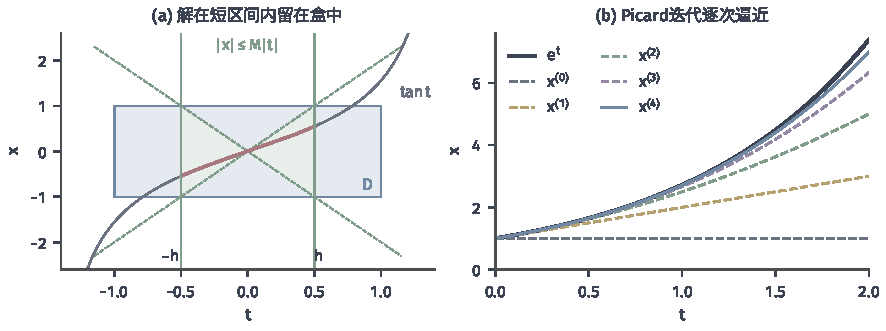
\includegraphics[width=150mm]{figures/03-optimization-evolution-and-signals/02-processes-and-trajectory-evolution/matplotlib/ode-picard/figure.pdf}
  \caption{局部存在性的两个画面。(a)方程$\dot x=1+x^2$，$x(0)=0$：蓝色矩形是$D=[-1,1]\times[-1,1]$，其中$|\dot x|\leq M=2$；绿色虚线是斜率$\pm M$的锥面，任何解在离开矩形之前都被限制在锥内。取$h=\min(a,b/M)=0.5$，红色的真解$\tan t$在$|t|\leq h$上留在矩形中；灰色是$\tan t$在更大区间上的部分。(b)方程$\dot x=x$，$x(0)=1$的Picard迭代$x^{(0)},\ldots,x^{(4)}$（虚线到实线）与真解$e^t$（黑色粗线）。}
  \label{fig:ode-picard}
\end{figure*}

迭代是否总能收敛，收敛的极限是否唯一？关键在于映射$\mathcal T$是否在某个完备的曲线空间里把两条曲线的距离缩小。设$\bm g$关于状态满足Lipschitz条件，常数为$L$，即$\|\bm g(t,\bm x)-\bm g(t,\bm y)\|_2\leq L\|\bm x-\bm y\|_2$。对两条曲线$\bm z_1,\bm z_2$，
\[
  \begin{aligned}
  \bigl\|(\mathcal T\bm z_1)(t)-(\mathcal T\bm z_2)(t)\bigr\|_2
  &\leq\left|\int_{t_0}^tL\|\bm z_1(s)-\bm z_2(s)\|_2\,\mathrm ds\right|\\
  &\leq L|t-t_0|\,\sup_s\|\bm z_1(s)-\bm z_2(s)\|_2.
  \end{aligned}
\]
时间区间长度不超过$h$时，$\mathcal T$至少把一致距离缩小到原来的$Lh$倍；$Lh<1$便是压缩。完备度量空间上的压缩映射恰有一个不动点，并且从任意初始点出发的迭代都收敛到它，这就是压缩映射定理，可参考\BookChapterRef{chap:metric-spaces}{卷二“度量空间”章}。剩下的问题是让$\mathcal T$把一个完备集合映回自身。

\paragraph{在短时间的曲线空间里压缩}
向量场通常只在出发点附近有界、有Lipschitz常数，所以只能在一个盒子里工作。图~\ref{fig:ode-picard}(a)画出这个盒子：时间方向半宽$a$，状态方向半径$b$。若盒中$\|\bm g\|_2\leq M$，任何解在离开盒子之前，状态偏离$\bm x_0$的距离不超过$M|t-t_0|$，即被限制在斜率为$\pm M$的锥里。只要时间不超过$b/M$，锥就还在盒子之内，解没有机会离开。于是时间区间要同时满足两个限制：留在盒中需要$Mh\leq b$，压缩需要$Lh<1$。

为此先说明关于状态的局部条件。称$\bm g$在$I\times D$上关于状态\term{局部Lipschitz}，若每一点$(t,\bm x)$都有邻域$U$与常数$L_U$，使$U$中同一时刻的两点满足$\|\bm g(t,\bm y)-\bm g(t,\bm z)\|_2\leq L_U\|\bm y-\bm z\|_2$。若$\bm g$对状态有连续偏导数，它就是局部Lipschitz的：在以$\bm x$为心的闭球上，Jacobian矩阵的范数有界，中值不等式沿两点间的线段给出Lipschitz常数。摆的向量场$(p,-\sin q-cp)$以及一切多项式向量场都属于这种情形。

\begin{theorem}[局部存在唯一性]
  \label{thm:ode-picard-lindelof}
  设$a,b>0$，$R=[t_0-a,t_0+a]\times\{\bm x:\|\bm x-\bm x_0\|_2\leq b\}\subseteq I\times D$，$\bm g$在$R$上连续，并且存在$L\geq0$使$R$中同一时刻的两点满足$\|\bm g(t,\bm y)-\bm g(t,\bm z)\|_2\leq L\|\bm y-\bm z\|_2$。记$M=\max_R\|\bm g\|_2$，取$h>0$满足
  \[
    h\leq a,\qquad Mh\leq b,\qquad Lh<1.
  \]
  则在$J=[t_0-h,t_0+h]$上初值问题~\eqref{eq:ode-ivp}恰有一个解；并且对任何包含$t_0$的区间$J'\subseteq J$，$J'$上的解都等于这个解在$J'$上的限制。
\end{theorem}

\begin{proof}
  令$\mathcal X$为$J$上满足$\|\bm z(t)-\bm x_0\|_2\leq b$（对每个$t\in J$）的连续曲线全体，取一致距离$\|\bm z_1-\bm z_2\|_\infty=\max_{t\in J}\|\bm z_1(t)-\bm z_2(t)\|_2$。$J$上的连续曲线在一致距离下构成完备空间，$\mathcal X$是其中的闭子集，因而也完备。

  \emph{映回。}对$\bm z\in\mathcal X$，点$(s,\bm z(s))$都在$R$中，所以式~\eqref{eq:ode-picard-map}的被积函数连续且范数不超过$M$。于是$\mathcal T\bm z$连续，并且$\|(\mathcal T\bm z)(t)-\bm x_0\|_2\leq M|t-t_0|\leq Mh\leq b$，即$\mathcal T\bm z\in\mathcal X$。

  \emph{压缩。}对$\bm z_1,\bm z_2\in\mathcal X$，上一段之前的估计给出$\|\mathcal T\bm z_1-\mathcal T\bm z_2\|_\infty\leq Lh\|\bm z_1-\bm z_2\|_\infty$，而$Lh<1$。由压缩映射定理，$\mathcal T$在$\mathcal X$中恰有一个不动点$\bm x$，由引理~\ref{lem:ode-integral-equation}它是$J$上的解。

  \emph{任何解都在盒中。}设$\bm y$是$J'$上的解，只看$t\geq t_0$的一侧，另一侧对称。令$t^\ast$为使$\bm y$在$[t_0,t^\ast]$上留在闭球中的最大时刻（闭球与$\bm y$的连续性保证最大值取到）。若$t^\ast<\sup J'$，则在$[t_0,t^\ast]$上点$(s,\bm y(s))$都在$R$中，积分方程给出$\|\bm y(t^\ast)-\bm x_0\|_2\leq M(t^\ast-t_0)<Mh\leq b$。严格不等式与连续性说明$\bm y$在$t^\ast$之后的一小段时间仍在球内，与$t^\ast$的最大性矛盾。因此$\bm y$在整个$J'$上留在球中。

  \emph{唯一。}把$\mathcal X$与$\mathcal T$中的$J$换成$J'$，上述映回与压缩的论证不变，所以$J'$上的不动点唯一。$\bm y$与$\bm x$在$J'$上的限制都是这个不动点，故二者相等。
\end{proof}

条件$Lh<1$只是为了让一致距离直接收缩，并不是本质限制。换用加权距离$\|\bm z\|_{L}=\max_{t\in J}e^{-2L|t-t_0|}\|\bm z(t)\|_2$，同样的估计给出
\[
  \bigl\|(\mathcal T\bm z_1-\mathcal T\bm z_2)(t)\bigr\|_2
  \leq L\left|\int_{t_0}^te^{2L|s-t_0|}\,\mathrm ds\right|\,\|\bm z_1-\bm z_2\|_{L}
  \leq\frac12e^{2L|t-t_0|}\|\bm z_1-\bm z_2\|_{L},
\]
即$\mathcal T$在加权距离下总以因子$\tfrac12$压缩，不论$h$多大。所以局部解的存在时间只受$h\leq a$与$Mh\leq b$限制，也就是只受“解不能跑出盒子”的限制。图~\ref{fig:ode-picard}(a)中的方程$\dot x=1+x^2$取$a=b=1$，得$M=2$，$h=0.5$；真解$\tan t$在$|t|\leq0.5$上满足$|\tan t|\leq0.547<1$，确实留在盒内，而它在$t=\pi/2$处趋于无穷，说明局部结论不能随意扩大到长时间区间。

把连续性换成Carathéodory条件，同一证明几乎原样适用，只是把常数换成可积函数。

\begin{theorem}[可测输入下的局部存在唯一性]
  \label{thm:ode-caratheodory-local}
  设$\bm g$满足第~\ref{sec:ode-integral-form}小节的Carathéodory条件，并且对每个紧集$K\subseteq D$存在在$I$的有限闭子区间上可积的函数$\ell_K\geq0$，使$\|\bm g(t,\bm y)-\bm g(t,\bm z)\|_2\leq\ell_K(t)\|\bm y-\bm z\|_2$对几乎每个$t$与全部$\bm y,\bm z\in K$成立。则存在$h>0$，使初值问题在$[t_0-h,t_0+h]\cap I$上恰有一个Carathéodory解。
\end{theorem}

\begin{proof}
  取闭球$K=\{\bm x:\|\bm x-\bm x_0\|_2\leq b\}\subseteq D$及其上的$m_K,\ell_K$。由积分的绝对连续性，可取$h>0$使$\int_{t_0-h}^{t_0+h}m_K\leq b$且$\int_{t_0-h}^{t_0+h}\ell_K<1$。在定理~\ref{thm:ode-picard-lindelof}的证明中，用$\int m_K$代替$Mh$，用$\int\ell_K$代替$Lh$，映回、压缩与“任何解都在盒中”三步的不等式都照样成立；不动点由积分给出，因而绝对连续。
\end{proof}

开关暖气的例子满足这两个定理之一吗？温度模型的向量场$-0.2x+u(t)$对状态是全局Lipschitz的，常数$0.2$，而$u$分段常值、可测有界，所以定理~\ref{thm:ode-caratheodory-local}适用，示例~\ref{ex:ode-switched-heating}中的折线状曲线就是唯一的Carathéodory解。

\paragraph{只有连续性时：等待后离开}
Lipschitz条件不能简单删去。考虑
\[
  \dot x=\sqrt{|x|},\qquad x(0)=0.
\]
零函数满足方程与初值，是一个解。对任意$c\geq0$，曲线
\[
  x_c(t)=\begin{cases}0,&0\leq t\leq c,\\(t-c)^2/4,&t>c\end{cases}
\]
也是解：在$t>c$处$\dot x_c=(t-c)/2=\sqrt{x_c}$，在$t=c$处左右导数都是零。于是同一个初值有无穷多个解，它们在原点“等待”任意长时间后离开，如图~\ref{fig:ode-nonunique}所示。

\begin{figure}[htbp]
  \centering
  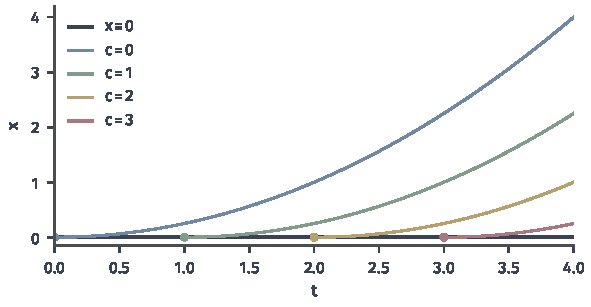
\includegraphics[width=100mm]{figures/03-optimization-evolution-and-signals/02-processes-and-trajectory-evolution/matplotlib/ode-nonunique/figure.pdf}
  \caption{方程$\dot x=\sqrt{|x|}$、$x(0)=0$的一族解。黑线是零解；彩色曲线是$x_c(t)=(t-c)^2/4$（$t>c$），在$c=0,1,2,3$之前停在原点（圆点标出离开时刻）。向量场连续，但在$x=0$处不满足Lipschitz条件。}
  \label{fig:ode-nonunique}
\end{figure}

问题出在原点附近。$\sqrt{|x|}/|x|=1/\sqrt{|x|}$在$x\to0$时无界，所以不存在包含原点的Lipschitz邻域。直观地说，向量场在原点为零，却在原点旁边以$\sqrt{|x|}$的速度推开状态；这个推力随距离缩小得太慢，使得从原点离开只需要有限时间。第~\ref{sec:ode-separable-linear}小节会用“时间等于路程除以速度的积分”把这个现象说得更清楚。若初值$x(0)=1$，则解在一段时间内远离原点，那里$\sqrt{x}$可微，定理~\ref{thm:ode-picard-lindelof}照样给出局部唯一性。

只要求连续时，存在性仍然成立：若$\bm g$在$(t_0,\bm x_0)$的邻域内连续，则初值问题至少有一个局部解。这就是Peano定理。证明的思路是用越来越细的Euler折线逼近解，这些折线在盒中有共同的斜率界$M$，因而一致有界、等度连续，由Arzelà--Ascoli定理可抽出一致收敛的子列，其极限满足积分方程\scite{math-hairer1993ode}。Peano定理只保证存在，正如上例所示，不保证唯一。本章后文的结论都建立在局部Lipschitz条件之上，Peano定理只作补充。

\subsection{最大解、延拓与爆炸}
\label{sec:ode-maximal-solutions}

本小节假设时间区间$I$是开区间，$\bm g$在$I\times D$上连续并关于状态局部Lipschitz。定理~\ref{thm:ode-picard-lindelof}在每个出发点附近给出局部解；现在问这些局部解能拼接成多长的一条。

\paragraph{用唯一性拼接局部解}
设$\bm x$定义在区间$J_1$上，$\bm y$定义在区间$J_2$上，二者都是同一初值问题的解。它们在公共区间$J_1\cap J_2$上必须相同。令$S=\{t\in J_1\cap J_2:\bm x(t)=\bm y(t)\}$。$S$包含$t_0$，并且由连续性在$J_1\cap J_2$中是闭集。$S$也是开集：若$\bm x(t_1)=\bm y(t_1)$，则$\bm x$与$\bm y$都是从$(t_1,\bm x(t_1))$出发的解，定理~\ref{thm:ode-picard-lindelof}说明它们在$t_1$附近的一个区间上相同。区间是连通的，既开又闭的非空子集只能是整个区间，所以$S=J_1\cap J_2$。

于是所有解可以无矛盾地拼在一起：把每个解的定义区间并起来，在并集的每一点上取任意一个在该点有定义的解的值。这样得到的曲线仍是解，而且任何解都是它的限制。

\begin{definition}[最大解]
  \label{def:ode-maximal-solution}
  初值问题的解$\bm x:J\to D$若不能延拓为更大区间上的解，称为\term{最大解}（maximal solution），$J$称为\term{最大存在区间}，记为$(\omega_-,\omega_+)$。
\end{definition}

最大存在区间是开区间：若它包含右端点$\omega_+<\sup I$，从$(\omega_+,\bm x(\omega_+))$出发的局部解就能把它再延长一段。若$\omega_+=\sup I$，解在整个未来都有定义，称为正向全局存在；若$(\omega_-,\omega_+)=I$，称为\term{全局解}。

\paragraph{有限时间爆炸}
光滑的向量场也可能只有有限的$\omega_+$。考虑
\[
  \dot x=x^2,\qquad x(0)=x_0>0.
\]
直接验算可知$x(t)=x_0/(1-x_0t)$是解，它在$t\uparrow1/x_0$时趋于无穷，所以$\omega_+=1/x_0$。初值越大，爆炸越早，见图~\ref{fig:ode-blowup}(a)。

\begin{figure*}[htbp]
  \centering
  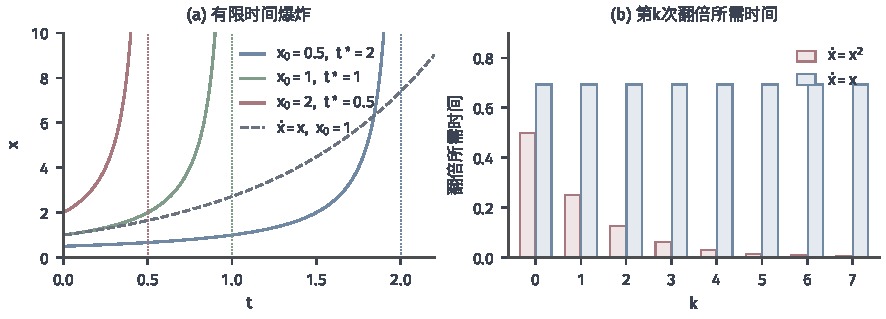
\includegraphics[width=150mm]{figures/03-optimization-evolution-and-signals/02-processes-and-trajectory-evolution/matplotlib/ode-blowup/figure.pdf}
  \caption{有限时间爆炸。(a)$\dot x=x^2$从$x_0=0.5,1,2$出发的解$x_0/(1-x_0t)$，点线标出爆炸时刻$t^\ast=1/x_0$；灰色虚线是$\dot x=x$、$x_0=1$的解$e^t$，对每个有限时刻都有定义。(b)从$x_0=1$出发，状态从$2^k$增长到$2^{k+1}$所需的时间：$\dot x=x^2$需要$1/2^{k+1}$，总和为$1$；$\dot x=x$每次都需要$\log2\approx0.693$，总和发散。}
  \label{fig:ode-blowup}
\end{figure*}

为什么$\dot x=x^2$会爆炸而$\dot x=x$不会？看状态每翻一番要花多少时间。速度为$x^2$时，从$X$走到$2X$所需时间是
\[
  \int_X^{2X}\frac{\mathrm d\xi}{\xi^2}=\frac1{2X},
\]
越往后翻倍越快；从$1$出发，所有翻倍时间之和$\tfrac12+\tfrac14+\cdots=1$有限，所以有限时间内要翻倍无穷多次。速度为$x$时，每次翻倍都需要$\int_X^{2X}\mathrm d\xi/\xi=\log2$，无穷多次翻倍需要无穷长时间。图~\ref{fig:ode-blowup}(b)把这两列时间并排画出。增长自我加速得足够快时，有限时间就能走完无限长的路。

解还可能以另一种方式停下来：没有趋于无穷，而是撞到状态集合的边界。取$D=(0,\infty)$，$\dot x=-1/x$，$x(0)=1$。由$\frac{\mathrm d}{\mathrm dt}x^2=2x\dot x=-2$得$x(t)=\sqrt{1-2t}$，它在$t\uparrow\tfrac12$时趋于$0$，速度$-1/x$却趋于$-\infty$；状态始终有界，但已经抵达$D$的边界，向量场在那里没有定义。两种情形的共同点是：轨迹终将离开$D$中的每个紧集。

\begin{theorem}[有限时间内离开每个紧集]
  \label{thm:ode-escape}
  设$I$为开区间，$\bm g$在$I\times D$上连续并关于状态局部Lipschitz，$\bm x$是最大解，最大存在区间为$(\omega_-,\omega_+)$。若$\omega_+<\sup I$，则对每个紧集$K\subseteq D$，存在$t_K<\omega_+$，使$\bm x(t)\notin K$对全部$t\in(t_K,\omega_+)$成立。特别地，$D=\mathbb R^d$时$\|\bm x(t)\|_2\to\infty$（$t\uparrow\omega_+$）。$\omega_-$一侧有对称的结论。
\end{theorem}

\begin{proof}
  先为$K$中的全部出发点找一个统一的局部存在时间。取$b>0$使$K_b=\{\bm y:\operatorname{dist}(\bm y,K)\leq b\}$仍是$D$中的紧集，取$a>0$使$T'=[t_0-a,\omega_++a]\subseteq I$。$\bm g$在紧集$T'\times K_b$上连续，因而有界，记上界为$M$。$\bm g$在这个紧集上关于状态还有统一的Lipschitz常数$L$：否则存在同一时刻的点对$(t_n,\bm y_n),(t_n,\bm z_n)$使差商超过$n$；由有界性$\|\bm y_n-\bm z_n\|_2\leq2M/n\to0$，抽子列使两列点收敛到同一点，那一点的Lipschitz邻域最终同时包含两列点，与差商超过$n$矛盾。

  于是对任意$s\in[t_0,\omega_+]$与$\bm\xi\in K$，盒子$[s-a,s+a]\times\{\|\bm y-\bm\xi\|_2\leq b\}$都在$T'\times K_b$中，定理~\ref{thm:ode-picard-lindelof}以统一的$h=\min\{a,b/M,1/(2L)\}$给出从$(s,\bm\xi)$出发、定义在$[s,s+h]$上的解。若某个$t_1\in(\omega_+-h,\omega_+)$使$\bm x(t_1)\in K$，从$(t_1,\bm x(t_1))$出发的解至少延续到$t_1+h>\omega_+$；由拼接论证，它与$\bm x$在公共区间上相同，二者合起来是超过$\omega_+$的解，与最大性矛盾。所以可取$t_K=\omega_+-h$。
\end{proof}

这个定理把“解能否延续”变成了“解是否留在某个紧集中”。只要事先知道轨迹在任意有限时间内都不会跑出某个紧集，最大解就延续到整个$I$。下面的Grönwall不等式正是得到这类先验界的工具。

\paragraph{Grönwall不等式}
设一个非负量$u(t)$的增长率不超过它自身的$b(t)$倍，即$\dot u\leq b(t)u$。把它与等号情形$\dot v=b(t)v$对比，后者的解是$v(t)=v(t_0)\exp\int_{t_0}^tb$，可以想见$u$不会超过这条指数包络。实际使用时，$u$常是两条轨迹之差的范数或状态的范数，它未必可微，能写出的只是积分形式的不等式。下面的引理处理积分形式。

\begin{lemma}[Grönwall积分不等式]
  \label{lem:ode-gronwall}
  \label{lem:action-state-gronwall}
  设$u$是$[t_0,T]$上的非负连续函数，$a\geq0$为常数，$b,r$是$[t_0,T]$上的非负可积函数（例如非负连续函数）。若对每个$t\in[t_0,T]$，
  \begin{equation}
    u(t)\leq a+\int_{t_0}^t\bigl(b(s)u(s)+r(s)\bigr)\,\mathrm ds,
    \label{eq:ode-gronwall-hypothesis}
  \end{equation}
  则对每个$t\in[t_0,T]$，
  \begin{equation}
    u(t)\leq a\exp\left(\int_{t_0}^tb(s)\,\mathrm ds\right)+\int_{t_0}^tr(s)\exp\left(\int_s^tb(\tau)\,\mathrm d\tau\right)\mathrm ds.
    \label{eq:ode-gronwall}
  \end{equation}
  特别地，$r=0$时$u(t)\leq a\exp\int_{t_0}^tb$；若进一步$a=0$，则$u\equiv0$。
\end{lemma}

\begin{proof}
  令$E(t)=a+\int_{t_0}^t(bu+r)$为式~\eqref{eq:ode-gronwall-hypothesis}的右端，则$u\leq E$。$E$是可积函数的不定积分，因而绝对连续，并且几乎处处有$\dot E=bu+r\leq bE+r$，这里用到$b\geq0$与$u\leq E$。令$B(t)=\int_{t_0}^tb$，$e^{-B}$也绝对连续，乘积法则几乎处处给出
  \[
    \frac{\mathrm d}{\mathrm dt}\bigl(E(t)e^{-B(t)}\bigr)=(\dot E-bE)e^{-B}\leq r\,e^{-B}.
  \]
  两个绝对连续函数之积仍绝对连续，可以由导数积分还原。从$t_0$积分到$t$，得$E(t)e^{-B(t)}\leq a+\int_{t_0}^tr(s)e^{-B(s)}\,\mathrm ds$。两边乘以$e^{B(t)}$，再用$u\leq E$，即得式~\eqref{eq:ode-gronwall}。
\end{proof}

$a=0$的特殊情形最常用来证明某个量恒为零：若非负连续的$u$满足$u(t)\leq\int_{t_0}^tb(s)u(s)\,\mathrm ds$，就只能$u\equiv0$。例如两条从同一初值出发的解，其差的范数$u$满足$u(t)\leq L\int_{t_0}^tu$，于是两条解相同；这是唯一性的另一种证明，而且不需要把时间区间缩短。

\paragraph{线性增长与全局存在}
$\dot x=x^2$爆炸，是因为速度的增长快于状态的线性函数。若向量场的大小至多随状态线性增长，Grönwall不等式就能阻止有限时间逃逸。

\begin{theorem}[线性增长下的全局存在]
  \label{thm:ode-global-existence}
  设$I$为开区间，$\bm g$在$I\times\mathbb R^d$上连续并关于状态局部Lipschitz，并且存在$I$上的非负连续函数$b,r$，使
  \[
    \|\bm g(t,\bm x)\|_2\leq b(t)\|\bm x\|_2+r(t)\qquad\text{对全部}(t,\bm x)\in I\times\mathbb R^d.
  \]
  则每个初值问题的最大解都在整个$I$上有定义。
\end{theorem}

\begin{proof}
  只证正向，反向相同。设$\omega_+<\sup I$。在$[t_0,\omega_+)$上，积分方程与增长条件给出
  \[
    \|\bm x(t)\|_2\leq\|\bm x_0\|_2+\int_{t_0}^{\omega_+}r+\int_{t_0}^tb(s)\|\bm x(s)\|_2\,\mathrm ds.
  \]
  $b,r$在紧区间$[t_0,\omega_+]$上连续，因而有界。对每个$T<\omega_+$在$[t_0,T]$上应用引理~\ref{lem:ode-gronwall}（取$r=0$，常数$a$为前两项之和），得$\|\bm x(t)\|_2\leq a\exp\int_{t_0}^{\omega_+}b$，右端与$T$无关。于是$\bm x$在$[t_0,\omega_+)$上留在一个闭球中，与定理~\ref{thm:ode-escape}矛盾。
\end{proof}

若$\bm g$关于状态全局Lipschitz，常数为$L$，则$\|\bm g(t,\bm x)\|_2\leq\|\bm g(t,\bm0)\|_2+L\|\bm x\|_2$，增长条件自动成立。摆的向量场$(p,-\sin q-cp)$的Jacobian矩阵为$\begin{bmatrix}0&1\\-\cos q&-c\end{bmatrix}$，其范数有统一上界，所以摆的每条轨迹都对全部时间存在。系数$\bm A(t),\bm b(t)$在$I$上连续的线性方程同样满足增长条件，解在整个$I$上存在。

增长条件只是充分条件。Logistic方程$\dot x=x(1-x)$的右端按$x^2$增长，可是从$x_0\in[0,1]$出发的解永远留在$[0,1]$中：$x\equiv0$和$x\equiv1$都是解，而拼接论证说明两条不同的解不能在同一时刻取同一值，所以一维自治方程的解不能穿过常值解。留在紧集$[0,1]$中的解由定理~\ref{thm:ode-escape}对全部时间存在。对$x_0>1$，正向解单调下降到$1$，也全局存在；反向时刻的解却在有限时间内趋于$+\infty$。状态集合有边界时，也要用同样的方式检查轨迹是否留在域内，例如浓度模型须说明从正值出发的状态不会变为负值。

\subsection{初值、输入与参数的连续依赖}
\label{sec:ode-continuous-dependence}

\paragraph{把差别送进积分方程}
测量初温时有误差，暖气的实际功率与标称值不同，模型中的散热系数也只是估计。若这些小差别会让一小时后的温度完全不同，模型就无法用于预测。下面把三种差别放进同一个估计：两条轨迹分别由$(\bm x_0,\bm u,\bm f)$与$(\widetilde{\bm x}_0,\widetilde{\bm u},\widetilde{\bm f})$产生，在积分方程中逐项相减。

\begin{theorem}[有限时间连续依赖]
  \label{thm:ode-continuous-dependence}
  设$\bm x,\widetilde{\bm x}:[t_0,T]\to D$分别是
  \[
    \dot{\bm x}=\bm f(t,\bm x,\bm u(t)),\ \bm x(t_0)=\bm x_0
    \qquad\text{与}\qquad
    \dot{\widetilde{\bm x}}=\widetilde{\bm f}(t,\widetilde{\bm x},\widetilde{\bm u}(t)),\ \widetilde{\bm x}(t_0)=\widetilde{\bm x}_0
  \]
  的解，并且两条轨迹都留在集合$K\subseteq D$中。设存在常数$L,L_u\geq0$与可积函数$\rho\geq0$，使对$t\in[t_0,T]$、$\bm y,\bm z\in K$以及输入所取的值$\bm v,\bm w$，
  \[
    \begin{aligned}
      \|\bm f(t,\bm y,\bm v)-\bm f(t,\bm z,\bm v)\|_2&\leq L\|\bm y-\bm z\|_2,\\
      \|\bm f(t,\bm y,\bm v)-\bm f(t,\bm y,\bm w)\|_2&\leq L_u\|\bm v-\bm w\|_2,\\
      \|\bm f(t,\bm y,\bm v)-\widetilde{\bm f}(t,\bm y,\bm v)\|_2&\leq\rho(t).
    \end{aligned}
  \]
  则对每个$t\in[t_0,T]$，
  \begin{equation}
    \begin{aligned}
    \|\bm x(t)-\widetilde{\bm x}(t)\|_2
    \leq{}&e^{L(t-t_0)}\|\bm x_0-\widetilde{\bm x}_0\|_2\\
    &+\int_{t_0}^te^{L(t-s)}\bigl(L_u\|\bm u(s)-\widetilde{\bm u}(s)\|_2+\rho(s)\bigr)\,\mathrm ds.
    \end{aligned}
    \label{eq:ode-continuous-dependence}
  \end{equation}
\end{theorem}

\begin{proof}
  两个积分方程相减，把被积函数之差拆成三段：
  \[
    \begin{aligned}
    \bm f(s,\bm x,\bm u)-\widetilde{\bm f}(s,\widetilde{\bm x},\widetilde{\bm u})
    ={}&\bigl[\bm f(s,\bm x,\bm u)-\bm f(s,\widetilde{\bm x},\bm u)\bigr]\\
    &+\bigl[\bm f(s,\widetilde{\bm x},\bm u)-\bm f(s,\widetilde{\bm x},\widetilde{\bm u})\bigr]\\
    &+\bigl[\bm f(s,\widetilde{\bm x},\widetilde{\bm u})-\widetilde{\bm f}(s,\widetilde{\bm x},\widetilde{\bm u})\bigr],
    \end{aligned}
  \]
  其中各量都在时刻$s$取值。三项依次不超过$L\|\bm x(s)-\widetilde{\bm x}(s)\|_2$、$L_u\|\bm u(s)-\widetilde{\bm u}(s)\|_2$与$\rho(s)$。于是$e(t)=\|\bm x(t)-\widetilde{\bm x}(t)\|_2$满足引理~\ref{lem:ode-gronwall}的假设，其中$a=\|\bm x_0-\widetilde{\bm x}_0\|_2$，$b\equiv L$，$r=L_u\|\bm u-\widetilde{\bm u}\|_2+\rho$。代入式~\eqref{eq:ode-gronwall}即得结论。
\end{proof}

式~\eqref{eq:ode-continuous-dependence}的三项对应三种误差来源：初值误差在开始时注入一次，此后最多按$e^{L(t-t_0)}$放大；输入误差和模型误差在每个时刻$s$持续注入，各自经过剩余时间$t-s$的放大后累计起来。三者来源不同，却都经过同一个传播因子。

定理要求两条轨迹都留在共同的集合$K$中，这是把局部条件用于全局比较时必须付出的代价。若向量场只是局部Lipschitz，可以取$K$为名义轨迹周围半径为$b$的闭管道，它是紧集，因而有统一的常数$L$。只要式~\eqref{eq:ode-continuous-dependence}右端在$[t_0,T]$上小于$b$，扰动后的轨迹就不可能离开这个管道：在它第一次触到管道边界之前，估计都成立，而估计说明它离名义轨迹的距离严格小于$b$。所以初值、输入和模型的扰动足够小时，扰动解在整个$[t_0,T]$上存在，并满足同一估计。

\paragraph{轨迹管}
图~\ref{fig:ode-trajectory-tube}把这个估计画成一束轨迹。对无阻尼摆$\dot q=p$，$\dot p=-\sin q$，Jacobian矩阵$\begin{bmatrix}0&1\\-\cos q&0\end{bmatrix}$的谱范数不超过$1$，所以可取$L=1$。从半径$0.05$的小圆上取$24$个初值，整束轨迹在$t\leq8$内的最大偏差被$0.05e^t$控制；$t=8$时这个上界约为$149$，比相平面本身还大。实际偏差小得多：圆心在$(0,1.2)$时，$t=8$的最大偏差只有约$0.11$。

\begin{figure*}[htbp]
  \centering
  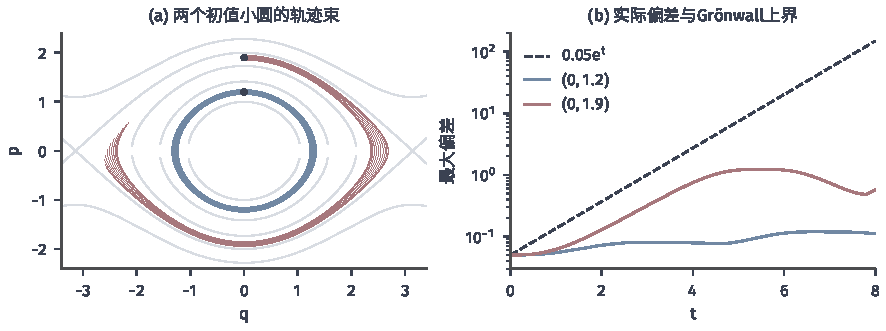
\includegraphics[width=150mm]{figures/03-optimization-evolution-and-signals/02-processes-and-trajectory-evolution/matplotlib/ode-trajectory-tube/figure.pdf}
  \caption{初值扰动的轨迹管。方程为无阻尼摆$\dot q=p$，$\dot p=-\sin q$，取$L=1$。(a)两个半径$0.05$的初值圆，圆心分别为$(0,1.2)$（蓝）与$(0,1.9)$（红），各取$24$个初值计算到$t=8$；浅灰曲线是能量等值线。(b)这些轨迹与圆心轨迹的最大欧氏距离（对数纵轴），黑色虚线是定理~\ref{thm:ode-continuous-dependence}的上界$0.05e^t$。}
  \label{fig:ode-trajectory-tube}
\end{figure*}

两束轨迹的表现不同，原因在于摆动周期依赖能量。圆心在$(0,1.9)$时，状态接近能把摆推过顶点的临界能量，周期对能量非常敏感：小圆上能量稍高的点转得慢、稍低的点转得快，轨迹束沿着能量等值线被拉成细长的弧。圆心在$(0,1.2)$时周期对能量不太敏感，轨迹束几乎保持原状。Grönwall上界只用到Lipschitz常数，无法区分这两种情形，它给出的是最坏情况的保证。

上界也看不出向量场的方向。温度模型$\dot x=-\lambda x+u$的Lipschitz常数是$\lambda$，若两条轨迹的初值相同，而加热量相差常数$\delta u$，式~\eqref{eq:ode-continuous-dependence}给出$|x-\widetilde x|\leq\delta u\,(e^{\lambda t}-1)/\lambda$，随时间指数增长。实际的差$x-\widetilde x$满足$\dot e=-\lambda e+\delta u$、$e(0)=0$，所以$e(t)=\delta u\,(1-e^{-\lambda t})/\lambda$，始终不超过$\delta u/\lambda$。散热把差别往回拉，Lipschitz常数只记录了“拉力的大小”，没有记录“往哪个方向拉”。利用方向得到不随时间增长的界，是第~\ref{sec:ode-stability}节的任务；在有限时间内，式~\eqref{eq:ode-continuous-dependence}已经足以说明解对数据连续依赖。

\paragraph{变分方程与灵敏度}
连续依赖说明误差可控；若向量场可微，还可以问误差的一阶近似是什么。设向量场依赖一组参数$\bm\theta\in\Theta\subseteq\mathbb R^k$（$\Theta$为开集），写$\bm g(t,\bm x,\bm\theta)$，并以$\bm x(t;\bm\xi,\bm\theta)$记从$\bm x(t_0)=\bm\xi$出发的解。初值或参数作一个小改变$\delta\bm\xi$、$\delta\bm\theta$，解的改变量近似为$\bm S(t)\delta\bm\xi+\bm s(t)\delta\bm\theta$，其中
\[
  \bm S(t)=\frac{\partial\bm x(t;\bm\xi,\bm\theta)}{\partial\bm\xi}\in\mathbb R^{d\times d},\qquad
  \bm s(t)=\frac{\partial\bm x(t;\bm\xi,\bm\theta)}{\partial\bm\theta}\in\mathbb R^{d\times k}
\]
称为\term{灵敏度矩阵}（sensitivity matrix）。它们本身满足线性微分方程。

\begin{theorem}[变分方程]
  \label{thm:ode-variational-equation}
  设$\bm g$在$I\times D\times\Theta$上连续，关于$\bm x$与$\bm\theta$有连续偏导数。则在解的存在区间上，$\bm x(t;\bm\xi,\bm\theta)$关于$(\bm\xi,\bm\theta)$连续可微，并且沿该解
  \begin{equation}
    \dot{\bm S}=\partial_{\bm x}\bm g\,\bm S,\quad\bm S(t_0)=\bm I;\qquad
    \dot{\bm s}=\partial_{\bm x}\bm g\,\bm s+\partial_{\bm\theta}\bm g,\quad\bm s(t_0)=\bm0,
    \label{eq:ode-variational-equation}
  \end{equation}
  其中$\partial_{\bm x}\bm g$与$\partial_{\bm\theta}\bm g$在$(t,\bm x(t;\bm\xi,\bm\theta),\bm\theta)$处取值。
\end{theorem}

解对初值和参数可微是标准结论，其证明对差商应用定理~\ref{thm:ode-continuous-dependence}一类的估计\scite{math-hairer1993ode}；这里引用它，只推导方程本身。对积分方程$\bm x(t)=\bm\xi+\int_{t_0}^t\bm g(s,\bm x(s),\bm\theta)\,\mathrm ds$关于$\bm\xi$求导，链式法则给出$\bm S(t)=\bm I+\int_{t_0}^t\partial_{\bm x}\bm g\,\bm S(s)\,\mathrm ds$；关于$\bm\theta$求导，$\bm\xi$不依赖$\bm\theta$，得$\bm s(t)=\int_{t_0}^t(\partial_{\bm x}\bm g\,\bm s+\partial_{\bm\theta}\bm g)\,\mathrm ds$。再对$t$求导就是式~\eqref{eq:ode-variational-equation}。$\bm S$的方程正是把原方程沿解线性化：初值的小扰动按沿途的Jacobian矩阵传播。

\begin{example}[散热系数的灵敏度]
  \label{ex:ode-temperature-sensitivity}
  温度模型$\dot x=-\lambda x+u$，取$x(0)=0$，$u=0.4$，参数$\theta=\lambda=0.2$。解为$x(t)=(u/\lambda)(1-e^{-\lambda t})$。由式~\eqref{eq:ode-variational-equation}，$s=\partial x/\partial\lambda$满足$\dot s=-\lambda s-x$，$s(0)=0$。直接对解求导也可得到
  \[
    s(t)=-\frac u{\lambda^2}\bigl(1-e^{-\lambda t}\bigr)+\frac u\lambda\,t\,e^{-\lambda t},
  \]
  代入可验证它满足上述方程。在$t=5$处，$s(5)=-10(1-e^{-1})+10e^{-1}\approx-2.642$。若散热系数增加$0.01$，五分钟时的温差约降低$0.0264$；实际重算$\lambda=0.21$得$x(5)\approx1.2382$，比$\lambda=0.2$时的$1.2642$低$0.0260$，与一阶近似一致。
\end{example}

训练含连续时间动态的模型时，损失对参数的梯度正是通过这类灵敏度，或与之等价的伴随方程计算的\scite{pgm-generative-chen2018}。需要注意，灵敏度描述的是有限时间内的局部一阶变化，与长期稳定是两件事：无阻尼摆的$\bm S(t)$一般随时间增长，轨迹却并不发散；阻尼摆的$\bm S(t)$最终趋于零，但这是第~\ref{sec:ode-stability}节要用稳定性理论证明的事。

\subsection{演化映射与流}
\label{sec:ode-flows}

\paragraph{解映射与复合关系}
在存在唯一的条件下，每个出发时刻$s$和出发状态$\bm\xi$决定一条最大解。把它在时刻$t$的值记作
\[
  \bm\varphi_{t,s}(\bm\xi)=\bm x(t),\qquad\text{其中}\bm x\text{是满足}\bm x(s)=\bm\xi\text{的最大解},
\]
它对最大存在区间$J(s,\bm\xi)$中的每个$t$有定义。固定$t,s$，$\bm\varphi_{t,s}$是从时刻$s$的状态到时刻$t$的状态的映射，称为\term{演化映射}（evolution map）。本章后面的状态转移矩阵、灵敏度矩阵和数值方法的误差分析，都是在研究这个映射。

\begin{theorem}[演化映射的复合]
  \label{thm:ode-evolution-composition}
  设$\bm g$连续并关于状态局部Lipschitz。若$s,t\in J(r,\bm\xi)$，则$\bm\varphi_{t,s}\bigl(\bm\varphi_{s,r}(\bm\xi)\bigr)=\bm\varphi_{t,r}(\bm\xi)$，并且$J\bigl(s,\bm\varphi_{s,r}(\bm\xi)\bigr)=J(r,\bm\xi)$。特别地，$\bm\varphi_{r,s}\bigl(\bm\varphi_{s,r}(\bm\xi)\bigr)=\bm\xi$。
\end{theorem}

\begin{proof}
  曲线$t\mapsto\bm\varphi_{t,r}(\bm\xi)$是最大解，并在时刻$s$经过$\bm\eta=\bm\varphi_{s,r}(\bm\xi)$。从$(s,\bm\eta)$出发的最大解是唯一的，拼接论证说明它与这条曲线有相同的定义区间并处处相同。于是$\bm\varphi_{t,s}(\bm\eta)=\bm\varphi_{t,r}(\bm\xi)$。取$t=r$得最后一式。
\end{proof}

图~\ref{fig:ode-flow-composition}画出这件事：从$r$走到$s$，再从$s$走到$t$，与直接从$r$走到$t$到达同一个状态。原因只是“这三点在同一条解上”，而这又来自唯一性。若解不唯一，例如$\dot x=\sqrt{|x|}$，从原点出发走到$s$后，下一步可以接任何一条等待后离开的解，复合关系便失去意义。

\begin{figure}[htbp]
  \centering
  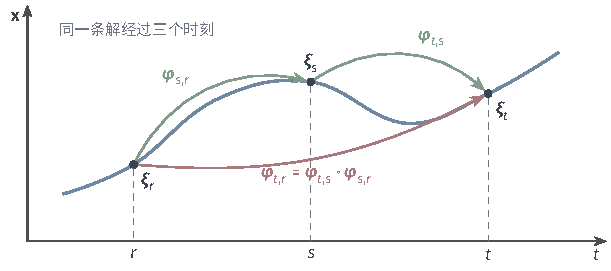
\includegraphics[width=100mm]{figures/03-optimization-evolution-and-signals/02-processes-and-trajectory-evolution/tikz/ode-flow-composition/figure.pdf}
  \caption{演化映射的复合关系示意。蓝色曲线是一条解在$(t,\bm x)$平面中的图像，它在时刻$r<s<t$分别经过$\bm\xi_r,\bm\xi_s,\bm\xi_t$。绿色箭头表示分两段传播$\bm\varphi_{s,r}$与$\bm\varphi_{t,s}$，红色箭头表示一次传播$\bm\varphi_{t,r}$；三者到达同一状态，是因为解唯一。}
  \label{fig:ode-flow-composition}
\end{figure}

\paragraph{自治方程的流}
向量场不显含时间时，规律不随时间改变，所以从$s$出发走$\tau$时间，与从$0$出发走$\tau$时间结果相同：若$\bm x$是从$(0,\bm\xi)$出发的解，则$\bm y(t)=\bm x(t-s)$满足$\dot{\bm y}(t)=\bm g(\bm y(t))$、$\bm y(s)=\bm\xi$，由唯一性它就是从$(s,\bm\xi)$出发的解。于是$\bm\varphi_{t,s}=\bm\varphi_{t-s,0}$只依赖时间差。

\begin{definition}[流]
  \label{def:ode-flow}
  设自治向量场$\bm g:D\to\mathbb R^d$局部Lipschitz，$J(\bm\xi)$是从$\bm x(0)=\bm\xi$出发的最大存在区间。映射$(t,\bm\xi)\mapsto\bm\varphi_t(\bm\xi)=\bm\varphi_{t,0}(\bm\xi)$（$t\in J(\bm\xi)$）称为$\bm g$的（局部）\term{流}。它满足$\bm\varphi_0=\mathrm{id}$，并在两边有定义时满足
  \begin{equation}
    \bm\varphi_{t+s}=\bm\varphi_t\circ\bm\varphi_s.
    \label{eq:ode-flow-group}
  \end{equation}
\end{definition}

式~\eqref{eq:ode-flow-group}由定理~\ref{thm:ode-evolution-composition}与时间平移得到。非自治方程没有这样的结构：$\dot x=tx$的解为$x(t)=\xi e^{(t^2-s^2)/2}$，于是$\bm\varphi_{1,0}(1)=e^{1/2}$，而同样经过一个单位时间的$\bm\varphi_{2,1}(1)=e^{3/2}$。规律本身随时间变化，传播效果就同时依赖起止两个时刻。

\paragraph{流把一团初值整体搬运}
固定$t$，流$\bm\varphi_t$把整个状态空间的点同时往前推$t$时间。与其一条一条地看轨迹，不如看一团初值被推成了什么形状。图~\ref{fig:ode-flow-deformation}从以$(-1,0)$为心、半径$0.35$的圆盘出发，画出它在$t=1.5,3,4.5$时的像。无阻尼摆把圆盘拉长、弯曲，但面积始终是$0.3848$，与初始圆盘相同；阻尼摆把圆盘越压越小，面积依次约为$0.2112$、$0.1159$、$0.0636$，恰好按$e^{-0.4t}$缩小。

\begin{figure*}[htbp]
  \centering
  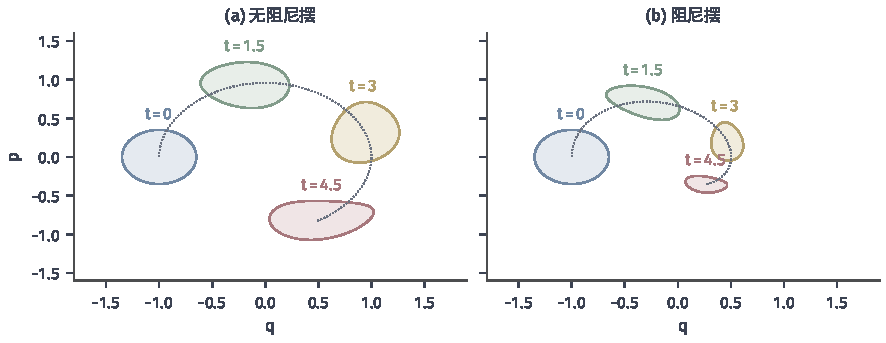
\includegraphics[width=150mm]{figures/03-optimization-evolution-and-signals/02-processes-and-trajectory-evolution/matplotlib/ode-flow-deformation/figure.pdf}
  \caption{流把一团初值整体搬运。初始集合是以$(-1,0)$为心、半径$0.35$的圆盘（蓝），依次画出它在$t=1.5$（绿）、$3$（黄）、$4.5$（红）时的像，点线是圆心的轨迹；边界由$400$个点分别积分得到。(a)无阻尼摆$\dot q=p$，$\dot p=-\sin q$：形状变化，面积保持$\pi\times0.35^2\approx0.3848$。(b)阻尼摆$\dot p=-\sin q-0.4p$：面积依次为$0.3848$、$0.2112$、$0.1159$、$0.0636$，与$0.3848e^{-0.4t}$一致。}
  \label{fig:ode-flow-deformation}
\end{figure*}

面积的变化由灵敏度矩阵控制。$\bm\varphi_t$在$\bm\xi$处的Jacobian矩阵就是定理~\ref{thm:ode-variational-equation}中的$\bm S(t)$，小区域的面积按$|\det\bm S(t)|$缩放。$\bm S$满足线性方程$\dot{\bm S}=\partial_{\bm x}\bm g\,\bm S$，第~\ref{sec:ode-time-varying-linear}小节将对这类方程证明$\det\bm S(t)=\exp\int_0^t\operatorname{tr}\partial_{\bm x}\bm g$。摆的$\partial_{\bm x}\bm g$的迹恒为$-c$，所以面积按$e^{-ct}$变化；无阻尼时迹为零，面积保持。这个观察是第~\ref{sec:ode-hamiltonian}节的起点。

\paragraph{局部流、正向全局与双向全局}
流是否对全部时间有定义，取决于最大存在区间。$\dot x=x^2$在$\xi>0$时$J(\xi)=(-\infty,1/\xi)$，在$\xi<0$时$J(\xi)=(1/\xi,\infty)$；对任何固定的$t>0$，$\bm\varphi_t$只在$\xi<1/t$上有定义，这种流称为局部流。

$\dot x=-x^3$的情形更微妙。由$\frac{\mathrm d}{\mathrm dt}x^{-2}=2$得$x(t)=\xi/\sqrt{1+2\xi^2t}$，它对全部$t\geq0$有定义，所以$\bm\varphi_t$对每个$t\geq0$在整条实轴上有定义，称为正向全局存在。反向时刻却只能退到$t>-1/(2\xi^2)$。经过时间$t$后，全部状态被压进区间$|x|<1/\sqrt{2t}$；这个区间之外的状态不是任何初值在$t$时间后的像。所以从$\bm\varphi_t(\xi)$恢复$\xi$总是可以的，只要沿原轨迹倒退；但随便指定一个状态往回推$t$时间，却可能在途中爆炸。逆向恢复需要相应方向的存在唯一。

若每个初值的最大解都在$(-\infty,\infty)$上存在，称流为全局流。这时每个$\bm\varphi_t$都是$\mathbb R^d$到自身的双射，逆映射是$\bm\varphi_{-t}$；常系数线性方程和摆都属于这种情形。下一节的状态转移矩阵是线性方程演化映射的矩阵表示，灵敏度矩阵则是非线性演化映射的一阶近似。
